\documentclass[]{book}
\usepackage{lmodern}
\usepackage{amssymb,amsmath}
\usepackage{ifxetex,ifluatex}
\usepackage{fixltx2e} % provides \textsubscript
\ifnum 0\ifxetex 1\fi\ifluatex 1\fi=0 % if pdftex
  \usepackage[T1]{fontenc}
  \usepackage[utf8]{inputenc}
\else % if luatex or xelatex
  \ifxetex
    \usepackage{mathspec}
  \else
    \usepackage{fontspec}
  \fi
  \defaultfontfeatures{Ligatures=TeX,Scale=MatchLowercase}
\fi
% use upquote if available, for straight quotes in verbatim environments
\IfFileExists{upquote.sty}{\usepackage{upquote}}{}
% use microtype if available
\IfFileExists{microtype.sty}{%
\usepackage{microtype}
\UseMicrotypeSet[protrusion]{basicmath} % disable protrusion for tt fonts
}{}
\usepackage[margin=1in]{geometry}
\usepackage{hyperref}
\hypersetup{unicode=true,
            pdftitle={Lecture Notes for Biology of Wildlife Populations},
            pdfauthor={Andrew Tyre},
            pdfborder={0 0 0},
            breaklinks=true}
\urlstyle{same}  % don't use monospace font for urls
\usepackage{natbib}
\bibliographystyle{apalike}
\usepackage{color}
\usepackage{fancyvrb}
\newcommand{\VerbBar}{|}
\newcommand{\VERB}{\Verb[commandchars=\\\{\}]}
\DefineVerbatimEnvironment{Highlighting}{Verbatim}{commandchars=\\\{\}}
% Add ',fontsize=\small' for more characters per line
\usepackage{framed}
\definecolor{shadecolor}{RGB}{248,248,248}
\newenvironment{Shaded}{\begin{snugshade}}{\end{snugshade}}
\newcommand{\KeywordTok}[1]{\textcolor[rgb]{0.13,0.29,0.53}{\textbf{{#1}}}}
\newcommand{\DataTypeTok}[1]{\textcolor[rgb]{0.13,0.29,0.53}{{#1}}}
\newcommand{\DecValTok}[1]{\textcolor[rgb]{0.00,0.00,0.81}{{#1}}}
\newcommand{\BaseNTok}[1]{\textcolor[rgb]{0.00,0.00,0.81}{{#1}}}
\newcommand{\FloatTok}[1]{\textcolor[rgb]{0.00,0.00,0.81}{{#1}}}
\newcommand{\ConstantTok}[1]{\textcolor[rgb]{0.00,0.00,0.00}{{#1}}}
\newcommand{\CharTok}[1]{\textcolor[rgb]{0.31,0.60,0.02}{{#1}}}
\newcommand{\SpecialCharTok}[1]{\textcolor[rgb]{0.00,0.00,0.00}{{#1}}}
\newcommand{\StringTok}[1]{\textcolor[rgb]{0.31,0.60,0.02}{{#1}}}
\newcommand{\VerbatimStringTok}[1]{\textcolor[rgb]{0.31,0.60,0.02}{{#1}}}
\newcommand{\SpecialStringTok}[1]{\textcolor[rgb]{0.31,0.60,0.02}{{#1}}}
\newcommand{\ImportTok}[1]{{#1}}
\newcommand{\CommentTok}[1]{\textcolor[rgb]{0.56,0.35,0.01}{\textit{{#1}}}}
\newcommand{\DocumentationTok}[1]{\textcolor[rgb]{0.56,0.35,0.01}{\textbf{\textit{{#1}}}}}
\newcommand{\AnnotationTok}[1]{\textcolor[rgb]{0.56,0.35,0.01}{\textbf{\textit{{#1}}}}}
\newcommand{\CommentVarTok}[1]{\textcolor[rgb]{0.56,0.35,0.01}{\textbf{\textit{{#1}}}}}
\newcommand{\OtherTok}[1]{\textcolor[rgb]{0.56,0.35,0.01}{{#1}}}
\newcommand{\FunctionTok}[1]{\textcolor[rgb]{0.00,0.00,0.00}{{#1}}}
\newcommand{\VariableTok}[1]{\textcolor[rgb]{0.00,0.00,0.00}{{#1}}}
\newcommand{\ControlFlowTok}[1]{\textcolor[rgb]{0.13,0.29,0.53}{\textbf{{#1}}}}
\newcommand{\OperatorTok}[1]{\textcolor[rgb]{0.81,0.36,0.00}{\textbf{{#1}}}}
\newcommand{\BuiltInTok}[1]{{#1}}
\newcommand{\ExtensionTok}[1]{{#1}}
\newcommand{\PreprocessorTok}[1]{\textcolor[rgb]{0.56,0.35,0.01}{\textit{{#1}}}}
\newcommand{\AttributeTok}[1]{\textcolor[rgb]{0.77,0.63,0.00}{{#1}}}
\newcommand{\RegionMarkerTok}[1]{{#1}}
\newcommand{\InformationTok}[1]{\textcolor[rgb]{0.56,0.35,0.01}{\textbf{\textit{{#1}}}}}
\newcommand{\WarningTok}[1]{\textcolor[rgb]{0.56,0.35,0.01}{\textbf{\textit{{#1}}}}}
\newcommand{\AlertTok}[1]{\textcolor[rgb]{0.94,0.16,0.16}{{#1}}}
\newcommand{\ErrorTok}[1]{\textcolor[rgb]{0.64,0.00,0.00}{\textbf{{#1}}}}
\newcommand{\NormalTok}[1]{{#1}}
\usepackage{longtable,booktabs}
\usepackage{graphicx,grffile}
\makeatletter
\def\maxwidth{\ifdim\Gin@nat@width>\linewidth\linewidth\else\Gin@nat@width\fi}
\def\maxheight{\ifdim\Gin@nat@height>\textheight\textheight\else\Gin@nat@height\fi}
\makeatother
% Scale images if necessary, so that they will not overflow the page
% margins by default, and it is still possible to overwrite the defaults
% using explicit options in \includegraphics[width, height, ...]{}
\setkeys{Gin}{width=\maxwidth,height=\maxheight,keepaspectratio}
\IfFileExists{parskip.sty}{%
\usepackage{parskip}
}{% else
\setlength{\parindent}{0pt}
\setlength{\parskip}{6pt plus 2pt minus 1pt}
}
\setlength{\emergencystretch}{3em}  % prevent overfull lines
\providecommand{\tightlist}{%
  \setlength{\itemsep}{0pt}\setlength{\parskip}{0pt}}
\setcounter{secnumdepth}{5}
% Redefines (sub)paragraphs to behave more like sections
\ifx\paragraph\undefined\else
\let\oldparagraph\paragraph
\renewcommand{\paragraph}[1]{\oldparagraph{#1}\mbox{}}
\fi
\ifx\subparagraph\undefined\else
\let\oldsubparagraph\subparagraph
\renewcommand{\subparagraph}[1]{\oldsubparagraph{#1}\mbox{}}
\fi

%%% Use protect on footnotes to avoid problems with footnotes in titles
\let\rmarkdownfootnote\footnote%
\def\footnote{\protect\rmarkdownfootnote}

%%% Change title format to be more compact
\usepackage{titling}

% Create subtitle command for use in maketitle
\newcommand{\subtitle}[1]{
  \posttitle{
    \begin{center}\large#1\end{center}
    }
}

\setlength{\droptitle}{-2em}
  \title{Lecture Notes for Biology of Wildlife Populations}
  \pretitle{\vspace{\droptitle}\centering\huge}
  \posttitle{\par}
  \author{Andrew Tyre}
  \preauthor{\centering\large\emph}
  \postauthor{\par}
  \predate{\centering\large\emph}
  \postdate{\par}
  \date{2016-12-27}

\usepackage{booktabs}

\let\BeginKnitrBlock\begin \let\EndKnitrBlock\end
\begin{document}
\maketitle

{
\setcounter{tocdepth}{1}
\tableofcontents
}
\chapter{Prerequisites}\label{prerequisites}

\chapter{The fundamental law of population
dynamics}\label{chap:fundamental}

\chapter{Making decisions}\label{chap:sdm}

In Chapter \ref{chap:fundamental} I defined a useful model as one that
helps a manager make a decision. This means that an understanding of the
process of decision making is fundamental to the process of modeling
population dynamics in an applied setting, at least. In this chapter I
introduce the concept of structured decision making, a simple framework
for making management decisions under risk and uncertainty.

I start with a simple example of a decision: whether or not to provide
supplemental food to a population of Hihi, an endangered bird in New
Zealand (Figure \ref{fig:hihi}). Managers at Kapiti Island want to
provide nectar feeders to support recently translocated Hihi because
they believe that the vegetation in the new location is not as rich in
nectar sources as the island from which they came. They believe that
additional food will support population growth in the translocated
population by either improving adult survival or the number of offspring
produced per pair. What they do not know is how much food to provide, or
whether some other aspect of the environment in Kapiti Island will limit
population growth despite increases in food availability. Concerns have
also been expressed that Hihi will become dependent on feeders, and
unable to utilize natural food sources.

\begin{Shaded}
\begin{Highlighting}[]
\NormalTok{knitr::}\KeywordTok{include_graphics}\NormalTok{(}\StringTok{"images/hihi_digitaltrails_cc_nc.jpg"}\NormalTok{)}
\end{Highlighting}
\end{Shaded}

\begin{figure}[htbp]
\centering
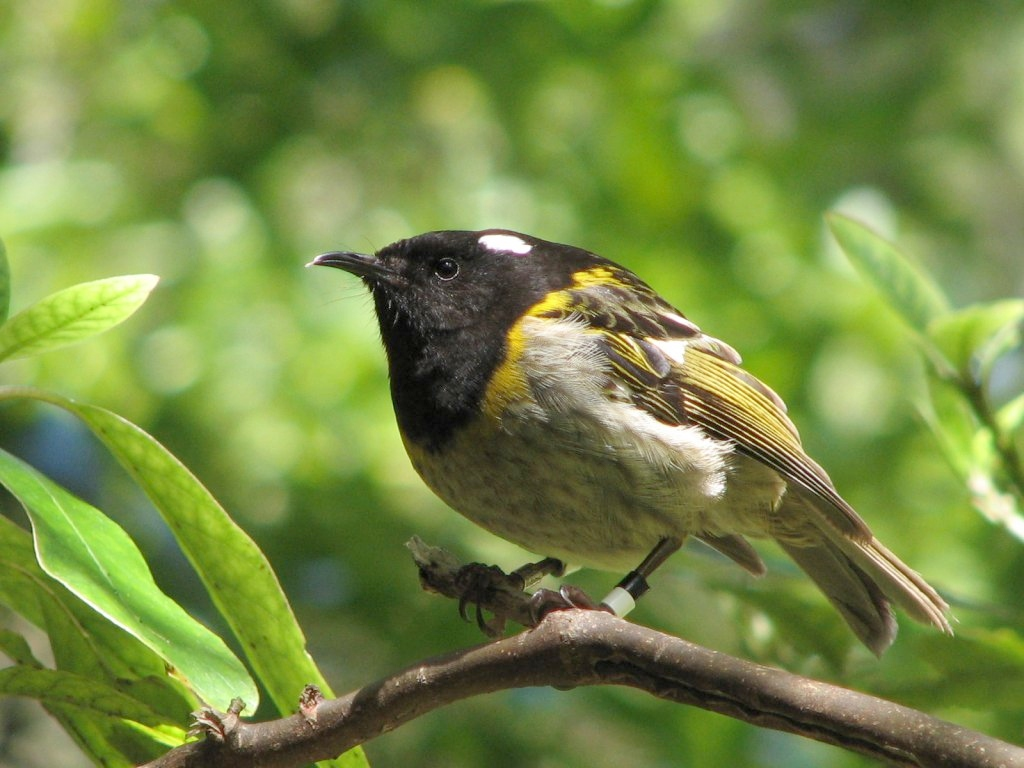
\includegraphics{images/hihi_digitaltrails_cc_nc.jpg}
\caption{\label{fig:hihi}The hihi, or stichbird. Image by digitaltrails.
\url{http://www.flickr.com/photos/digitaltrails/87192080/} (CC BY-NC-SA
2.0)}
\end{figure}

Although this is a relatively simple decision, it has all the features
that make decisions complicated and difficult. There are multiple
competing outcomes, multiple ways of reaching those outcomes, and
uncertainty about which actions will lead to which outcomes. In the face
of all this complexity, it is very human to avoid making a decision ---
which is itself a decision with outcomes --- and focus on acquiring more
information or attempting to pass responsibility for the decision
onwards. Research throughout the 20th century has documented the many
ways in which human cognition fails when faced with complex decisions.
Psychologists have also studied ways in which to help humans make
decisions in such circumstances. In this book I will introduce a simple
5 step approach to decision making (Smart Choices reference) that can
help overcome the psychological traps of decision making; it has a
simple easy to remember acronym PrOACT, reminding you to be proactive in
decision making. The five steps are: Problem, Objectives, Actions,
Consequences, Tradeoffs.

\section{Problem}\label{problem}

The first step in making a decision is to ensure that you are in fact
making the correct decision. What is the problem that has to be solved?
Who has to solve that problem? Correctly identifying both the problem
and the problem solver is critical to making a good decision. If the
problem you think you're trying to solve is in fact a decision at a
higher level of organization, then no matter how good your decision
making is you will not be able to solve the problem. Someone else is
making the decision. You may be able to advise that person, but that is
a very different role than directly making the decision yourself.

What is the problem to be solved in the Hihi example? Is it identifying
the direct effects of food supplementation on adult survival? What kind
of monitoring program should be in place? How many translocated
populations should receive food supplementation? All of these are
legitimate questions. The key to identifying the right problem to solve
is to focus on things that are under the control of the decision maker.
If the manager of Kapiti Island is the decision maker, then deciding
which translocated populations should receive food supplementation is
beyond her scope --- that will be decided by someone else. Similarly, a
management problem will typically involve a choice among alternatives,
rather than a resolution of an uncertainty. Identifying the direct
effects of food supplementation on adult survival, while potentially
useful information, does not involve a choice between alternatives by
the decision maker. Choosing what to monitor in the park, and how, is a
choice among alternatives -- there are many things that could be
measured. Similarly how many feeders and where to place them leads to
choices among alternatives by the manager of Kapiti Island.

Careful thought about who is making the decisions, and what decisions
they have to make, is a critical first step in problem solving, and
often the most neglected. The more effort devoted to this step the
better, although it is also possible to get bogged down at this stage.
Rather than attempting to solve all of the problems at once, it is
useful to tackle individual decisions completely, and sequentially.
Sometimes the solution to one problem turns out to depend on the
solution to a different problem -- the decisions are linked. Linked
decisions are more complex than decisions that can stand alone, but
breaking linked decisions into separate problems and tackling each
independently makes it easier. In the Hihi example, the choice about
what to monitor and how depends to a great extent on what choices are
made about feeding stations. So first laying out the feeding station
decision will provide a great deal of information about how to solve the
monitoring problem.

\section{Objectives}\label{objectives}

Once the problem has been (tentatively) decided on, the next step is to
determine how to measure success. The terms used for measuring success
vary widely, and different texts will argue for critieria, metrics,
goals, objectives, targets and many others besides. I will try to keep
it simple. An objective is an attribute of the system being managed that
has some value to the decision maker. In the Hihi example, the number of
adult Hihi in Kapiti Island is a measurable attribute. The annual adult
survival probability is another measurable attribute. The number of
feeding stations in the park is a measurable quantity as well. How do
you decide which and how many objectives are necessary?

One approach to this problem is to categorize the measurable quantities
into either means objectives or fundamental objectives. Distinguishing
between these two is relatively easy. For each putative objective, you
must ask yourself, ``why does this matter?''. If the answer is simply,
``because it does'', then the objective is likely a fundamental
objective. In contrast, if the answer is ``it helps achieve objective
X'', then it is a means objective --- a useful step, but not of interest
in and of itself.

Take a look at the quantity ``number of feeding stations in Kapiti
Island''. Does the manager care about this quantity? If there were no
Hihi, would having 5 or 10 stations be better than having none? If yes,
then the number of feeding stations would be fundamental --- more
feeding stations is better, regardless of what else is happening.
However, this seems unlikely. The only reason for feeding stations is to
help the Hihi population, so this is a means objective rather than a
fundamental objective.

In contrast, asking is 20 Hihi better than zero Hihi leads to a
different conclusion -- regardless of what else is happening in the
park, 20 Hihi are better than none. The population size of Hihi on
Kapiti Island seems like a fundamental objective, at least for this
decision. The adult survival probability is an example of a more
difficult objective. All other things equal, is a population with higher
survival better than a population with lower survival? Imagine that
there are 100 Hihi in the park, but you can have 100 birds with an
annual survival of 0.85, or 100 birds with an annual survival of 0.9.
Which is better? This is not so straightforward to sort out, and the
answer may well depend on other vital rates of the population, and how
they vary with population size. For example, what if the population of
100 with a low adult survival rate is only maintained by continued
immigration from another population? The population in Kapiti Island is
then a sink, and could be causing the larger metapopulation of Hihi to
be lower than it otherwise would.

This sort of complex interaction between potential objectives is not
uncommon in fisheries and wildlife management problems. A more nuanced
approach to the means vs.~fundamental dichotomy is to construct an
objectives hierarchy. Each potential objective is given a node, and then
connections are made between nodes in order to identify causal
relationships between them (see Figure @ref(fig:hihi\_objectives)).

\begin{Shaded}
\begin{Highlighting}[]
\NormalTok{knitr::}\KeywordTok{include_graphics}\NormalTok{(}\StringTok{"images/hihi_objectives_hierarchy.png"}\NormalTok{)}
\end{Highlighting}
\end{Shaded}

\begin{figure}
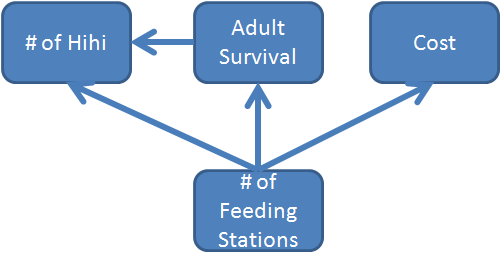
\includegraphics[width=6.96in]{images/hihi_objectives_hierarchy} \caption{An objectives hierarchy for the hihi feeding problem.}(\#fig:hihi_objectives)
\end{figure}

\section{Alternatives}\label{alternatives}

Once the objectives are described, the next step is to lay out all the
alternatives, the different possible choices that can be made. This step
is crucial, and requires creativity. It is all too easy at this stage to
fall into the trap of only specifying alternative outcomes that are
thought to be acceptable. The key is to lay out the broadest range of
alternatives possible --- even if you think some of them are impossible
to achieve. The subsequent exercise of evaluating the consequences and
tradeoffs will demonstrate which alternatives are impossible, but may
also help to identify new alternatives that had not been previously
considered. This is especially true for combinations of alternative
actions.

A good source for alternatives is to examine the lower end of the
objectives hierarchy -- those ``means objectives'' that are not ends in
themselves, but lead to improvements in the fundamental objectives. In
many instances these are attributes of the system that can be
manipulated, not just measured. In the Hihi feeding station problem, the
obvious place to start is with the number of feeding stations. This is
something that is under the control of the park manager. Keeping a broad
mind about the alternatives suggests we should consider everything from
placing no feeding stations to placing many more than have been tried in
the past. We should also consider alternatives about where to place the
stations. Hihi management also involves placing nestboxes, so feeders
should only be placed where there are nest boxes, but how many feeders
per nestbox? Should we put feeders with all nestboxes? Do we need to
maintain the feeders year round, or only during the breeding season?
Suddenly we have many more things that we can manipulate than we
expected! For the purposes of this example, let us define 5 alternatives
as combinations of 0, 1 or 2 feeders per nest box, and maintaining
feeders either year round or only in the breeding season. We end up with
5 alternatives, rather than 6, because 0 feeders per nest box doesn't
require choosing a duration of feeding.

\section{Consequences}\label{consequences}

Once we have our objectives and alternatives, the next step is to
articulate the consequences of each alternative for each objective. One
of our objectives is the number of Hihi, so this is the part where
modeling population dynamics comes in. In essence, we want to predict
what the population size will be in the future for each of our
alternatives. This step is also where we find out how much we really
know about the system we are trying to manage.

Predicting consequences doesn't have to be hard. For a first cut at a
problem, it can simply be a statement of what relevant experts think
will happen. Even ranking alternatives can be sufficient as a starting
point, and that can usually be done with relatively little information.

I started by assuming that no feeding stations would be the worst for
population size and adult survival, and of course, have the lowest cost
(Table @ref(tab:hihi\_con1)). I also assumed that having 2 feeding
stations per nest box would have the largest effect on population size,
and be the most expensive. Notice that all options are tied for adult
survival --- this is because further consulting with experts
(i.e.~reading) revealed that supplementary feeding affects reproduction
but not survival. That last observation led me to suppose that having 2
feeding stations only during the breeding season would have an equal
effect on population size as maintaining the stations year round, but
would of course be cheaper. By analogy then, having 1 feeding station
all year will be equivalent to 1 feeding station for the breeding
season, but both are less good than having 2 stations. Finally, I
assumed that having 2 feeding stations for the breeding season would
cost the same as having 1 station for the entire year, and having a
single station just for the breeding season was the cheapest next to
having no stations at all.

\begin{table}[tbp]
\caption{Prototype consequences table for the Hihi feeding problem.\label{tab:hihi_con1}}
\begin{tabular}{lrrr}
\toprule
   \textbf{Alternative}
  &\textbf{Cost}
  &\textbf{\# of Hihi}
  &\textbf{Adult Survival}
\\\midrule
   0 FS           & 1 & 1 & 1 
\\ 1 FS, all year & 3 & 2 & 1
\\ 2 FS, all year & 4 & 3 & 1
\\ 1 FS, breeding & 2 & 2 & 1
\\ 2 FS, breeding & 3 & 3 & 1
\\\bottomrule
\end{tabular}
\end{table}

\section{Tradeoffs}\label{tradeoffs}

The final step in the process is to examine the consequence table to
identify strategies or alternatives that perform the best. If you're
lucky, there's one alternative that beats all others. Most of the time,
you'll not be so lucky, and there will be some alternatives that win on
one objective, and others that win on a second objective. Somehow the
different objectives must be ``traded off'' against one another. There
are many ways of doing this, and for the most part these boil down to
weighting the objectives in some fashion. But before getting to that
level of complexity, it is always worthwhile to see if the decision
problem can be simplified.

The first tactic for simplification is to examine the objectives and see
if any of them are uninformative. An uninformative objective is one that
does not distinguish among the alternatives. If it isn't distinguishing
among the alternatives, then in effect it can be ignored. In the Hihi
problem adult survival is uninformative (Table @ref(tab:hihi\_con1)); it
has the same value for all alternatives. So we can simply remove it from
the consequences table, and proceed with a problem that is now much
simpler --- only 2 objectives to worry about instead of 3 (Table
@ref(tab:hihi\_con2)).

\begin{table}[tbp]
\caption{Consequences table for the Hihi feeding problem after simplifying by removing irrelevant objectives.\label{tab:hihi_con2}}
\begin{tabular}{lrr}
\toprule
   \textbf{Alternative}
  &\textbf{Cost}
  &\textbf{\# of Hihi}
\\\midrule
   0 FS           & 1 & 1 
\\ 1 FS, all year & 3 & 2 
\\ 2 FS, all year & 4 & 3 
\\ 1 FS, breeding & 2 & 2 
\\ 2 FS, breeding & 3 & 3 
\\\bottomrule
\end{tabular}
\end{table}

The second tactic for simplification is to look for strategies that are
``completely dominated'' by one or more other strategies. That is, the
alternative performs equal or worse on every single objective. For
example, take a look at the single feeding station for the entire year
alternative. It costs more (3 vs 2) and has the same effect on
population size (2 vs 2) as the single feeding station in the breeding
season alternative. So, in this simple prototype of the decision
problem, there would be no circumstances in which we would choose to run
the feeding station for the entire year. If there were, then that would
suggest that there is a fundamental objective that has not been
captured, or perhaps our ranking of alternative performance is
incorrect. In contrast, compare the no feeding stations alternative with
the single station for the breeding season alternative. No feeding
station is cheaper, but the single breeding season station does better
for population size. In this case, there is no way to eliminate one of
these alternatives --- we will be forced to trade off the cost against
the benefit to the population size.

A similar argument allows us to eliminate the alterative with 2 feeding
stations for the entire year --- it does not perform better in any
respect than 2 feeding stations just in the breeding season. We now have
a much simpler problem to look at --- just 3 alternatives and 2
objectives (Table 3). At this point we could try the 1st simplification
tactic again --- having eliminated some alternatives can leave some
objectives irrelevant to the remaining set. However, in this case we've
gone as far as simplification can get us. Now we need to do something
more complex. It turns out that one of the flaws of ranking alternatives
now comes back to bite us.

\begin{table}[tbp]
\caption{Consequences table for the Hihi feeding problem after simplifying by removing dominated alternatives.\label{tab:hihi_con3}}
\begin{tabular}{lrr}
\toprule
   \textbf{Alternative}
  &\textbf{Cost}
  &\textbf{\# of Hihi}
\\\midrule
   0 FS           & 1 & 1 
\\ 1 FS, breeding & 2 & 2 
\\ 2 FS, breeding & 3 & 3 
\\\bottomrule
\end{tabular}
\end{table}

Ranking destroys any information (or in this case, I never elicited that
information) about how far apart each alternative is on that objective.
For example, probably the biggest cost of maintaining the feeding
stations is the personnel needed to visit each station. However, in this
case, someone has to visit each nest box anyway to check for parasites.
So as long as visits to feeding stations don't need to happen more often
than visits to nest boxes, the cost difference between the no feeding
station alternative and the single station is not that great. In
contrast, the increase to having 2 feeding stations could be larger, as
now more material will have to be carried in rough terrain, and more
travel between feeding stations will be required. Exactly how we resolve
the tradeoffs between cost and population size benefits will depend a
great deal on details like this. But now, instead of trying to worry
about everything, we are very focused on the particular details that
distinguish the remaining alternatives from each other.

So let's fill in the table with some values that have meaningful units
on them. After some discussion, we decide that one feeding station
doesn't take extra time, but having 2 stations to visit will take an
extra hour, on average. We'll measure the population size relative to
the change obtained by putting in one feeding station, so the 1 feeding
station alternative gets a value of 1, and the value for 2 feeding
stations will give us the proportional improvement for a second feeding
station (Table @ref(tab:hihi\_con4)). Now we revisit our simplification
tactics, and we can see that the no feeding station alternative is
completely dominated by the single feeding station alternative. We're
really getting somewhere now! The problem has reduced down to
determining if an extra person-hour per week is worth a hypothesized
50\% increase in population size.

\begin{table}[tbp]
\caption{Consequences table for the Hihi feeding problem after converting consequences to meaningful units.\label{tab:hihi_con4}}
\begin{tabulary}{0.7\textwidth}{lRR}
\toprule
   \textbf{Alternative}
  &\textbf{Cost [extra person-hours/week]}
  &\textbf{Population size [increase relative to 1 feeding station]}
\\\midrule
   0 FS           & 0 & 0 
\\ 1 FS, breeding & 0 & 1 
\\ 2 FS, breeding & 1 & 1.5 
\\\bottomrule
\end{tabulary}
\end{table}

I added a new word to the description in the last paragraph:
hypothesized. This emphasizes something that we've so far ignored. To
some extent, all of the rankings and quantities that we used so far are
uncertain --- we do not know them exactly. And in many cases they will
in fact vary naturally --- the amount of work required to maintain one
or two feeding stations per nestbox probably varies by nestbox. The
terrain is different, the stations are harder to travel between, the
liquid in the feeding stations evaporates faster on warmer days, and so
on. This kind of variation can make a big difference when making
tradeoffs between objectives, because it introduces risk into the
equation. It is possible that we will not obtain the benefits we seek,
or that the costs will be higher.

In the case of the improvement in population size, I've hypothesized
that 2 feeding stations are better than one, but not twice as good. I'm
not very certain about that however; it could be as low as 1 (no
improvement at all) to as high as 2. There are many methods for
proceeding in the face of uncertainty like this, but for the moment, I
will stick with the point estimate. I feel that the extra benefit is not
worth the extra cost. As long as the population is increasing, I am
satisfied that we are meeting the overall goal, and therefore I choose
the less expensive alternative.

\BeginKnitrBlock{.rmdnote}
\subsection{Wild horses in the American Southwest}\label{wild-horses}

Wild horses have roamed the west since their re-introduction to North
America by the Spanish Conquistadors. Most of these horses occur on land
managed by the Bureau of Land Management, and since 1971 the Wild
Free-Roaming Horses and Burro's Act has stipulated what BLM can and
cannot do to manage this population. The BLM and other federal agencies
are supposed to monitor horse numbers, and ensure that they ``preserve
and maintain a thriving natural ecological balance.'' Although current
management targets a maximum population of 23,622 horses across 179
management units, the current free-roaming population exceeds 33,000.
Political pressure means that BLM is not able to cull horses, instead
relying on capture and adoption to reduce wild populations.
Unfortunately adoption demand is usually much less than the number of
horses captured, and as a result there is a burgeoning captive herd of
around 45,000 horses that must also be maintained. A few horses are
sold, but most remain in captivity until they die of natural causes.

Garrott and Oli (2013) worked out that the captive population would
stabilize around 60,000 horses by 2027 representing a balance between
natural deaths and new captures from the wild. Caring for these animals
will cost in excess of \$100 million dollars per year; the 2012 budget
for the Wild Horse and Burro program was \$74 million, of which 60\% is
used to care for captive horses.

A National Research Council report (NRC 2013) on wild horses and burros
concluded that if removals from the free-roaming population ceased, the
population would grow unchecked until food and water became limiting. At
that point the horses would be in poor health, and rangelands would be
degraded affected native species and other public uses (grazing,
hunting).

Garrott, R.A. and M.K. Oli (2013) A critical crossroad for BLM's Wild
Horse Program. Science, 341:847-848.

NRC (2013) Using Science to Improve the BLM Wild Horse and Burro
Program: A Way Forward. National Academies Press, Washington, DC.
\EndKnitrBlock{.rmdnote}

\section{Exercises}\label{exercises}

\begin{enumerate}
\def\labelenumi{\arabic{enumi}.}
\item
  See Table @ref(tab:muskox\_con1) for the consequences of a decision
  about how many Muskox to remove from Nunivak Island AK, identify all
  the alternatives that are completely dominated. How many objectives
  are redundant, which ones, and why?
\item
  Read the problem description in this note: \ref{wild-horses}. Draw up
  a proposed objectives hierarchy for the managers to consider.
\end{enumerate}

\begin{table}[tbp]
\caption{Consequences table for Muskox removal problem\label{tab:muskox_con1}}
\begin{tabulary}{0.7\textwidth}{lRRRR}
\toprule
   \textbf{Alternative}
  &\textbf{Cost [\$]}
  &\textbf{Range Condition}
  &\textbf{Total Population, April}
  &\textbf{Herd Sex ratio [males:females]}
\\\midrule
   None            & 0   & 0   & 750 & 56:44 
\\ 10\% of total   & 1   & 1   & 700 & 56:44
\\ 20\% of females & 2.5 & 1.5 & 500 & 70:30
\\ 20\% of total   & 2   & 1.2 & 600 & 56:44
\\\bottomrule
\end{tabulary}
\end{table}

\bibliography{packages,book}


\end{document}
